\documentclass{article}
\usepackage{arxiv}

\usepackage[utf8]{inputenc}
\usepackage[english, russian]{babel}
\usepackage[T1]{fontenc}
\usepackage{url}
\usepackage{booktabs}
\usepackage{amsfonts}
\usepackage{nicefrac}
\usepackage{microtype}
\usepackage{bm}
\usepackage{lipsum}
\usepackage{graphicx}
\usepackage{natbib}
\usepackage{doi}
\usepackage{mathtools}


\title{Декодирования сигналов головного мозга в аудиоданные}

\author{ Набиев Мухаммадшариф \\
        Кафедра интеллектуальных систем\\
	МФТИ\\
	\texttt{nabiev.mf@phystech.edu} \\
	\And
	Северилов Павел \\
	Кафедра интеллектуальных систем\\
	МФТИ\\
	\texttt{pseverilov@gmail.com} \\
}
\date{}

\renewcommand{\shorttitle}{Декодирование сигналов головного мозга а аудиоданные}

%%% Add PDF metadata to help others organize their library
%%% Once the PDF is generated, you can check the metadata with
%%% $ pdfinfo template.pdf
\hypersetup{
pdftitle={Декодирования сигналов головного мозга в аудиоданные},
pdfsubject={q-bio.NC, q-bio.QM},
pdfauthor={Набиев Мухаммадшариф, Северилов Павел},
pdfkeywords={First keyword, Second keyword, More},
}

\begin{document}
\maketitle

\begin{abstract}
В данной работе исследуется проблема декодирования сигналов головного мозга в аудиосигналы с использованием физически- информированных методов получения эмбеддингов сигналов. Предлагается решить задачу классификации стимулов по соответствующим сегментам аудиоданных. Под стимулом понимается аудиосигнал, который вызвал активность мозга, соответствующая ЭЭГ-сигналу. Данные для задачи представляют собой 183 пар вида аудиофрагмент и мозговая активность в виде ЭЭГ, который он вызвал. Продолжительность каждой записи составляет примерно 15 минут. В качестве критерия качества для выбора оптимальной модели используется средняя долей правильных ответов. Предлагается исследовать методы получения скрытых представлений, которые учитывают физические принципы, с целью улучшения качества обработки аудиосигналов и повышения точности их декодирования. Полученные результаты имеют важное значение для развития интерфейсов мозг-компьютер и понимания принципов обработки аудиосигналов человеческим мозгом.

\end{abstract}

\keywords{auditory EEG decoding \and natural speech processing \and EEG}

\section{Введение} 
    \par 
    Слух, одно из наиболее важных человеческих чувств, играет решающую роль в нашем повседневном взаимодействии с окружающим миром. Однако многие люди со всего мира сталкиваются с проблемами слуха, которые могут серьезно ограничить их способность воспринимать звуки окружающей среды. В свете этих проблем возникает интерес к исследованию взаимосвязи между звуком и мозговыми сигналами~\citep{audioeeg}. В данной области выделена задача декодирования мозговых сигналов в аудиоданные. 
    \par 
    Задачу декодирования можно поставить двумя способами: с помощью классификации и регрессии. В данной работе мы сконцентрируемся на задаче классификации. Требуется решить задачу мультиклассовой классификации, когда на вход подается ЭЭГ сигнал и $K$ стимулов, из которых только один соответствует сигналу. Под стимулом подразумевается сегмент аудио, который стимулировал сигнал в мозгу субъекта. 
    \par 
    Существует базовое решение этой задачи, использующее расширенную сверточную нейросеть~\citep{Accou2021ModelingTR}. Оно состоит из трех главных блоков: блок для пространственного преобразования ЭЭГ, энкодер для ЭЭГ и энкодер для стимула. Энкодеры ЭЭГ и стимула получают эмбеддинги путем свертки со расширенными ядрами. Далее считается близость представлений и определяется стимул.
    \par 
    Известна модификация базового решения с использованием многомерного внимания (Multi-head attention) и управляемого рекуррентного блока (Gated Recurrent Unit)~\citep{multihead-gru}. Также авторы генерируют спектрограмму для получения дополнительных признаков, как, например, частота. Спектрограмма проходит через управляемый рекуррентый блок, а уже потом подаются на вход в энкодер стимула. После получения скрытых представлений, аналогично базовому решению, считается близость.
    \par 
    В постановке классификации наиболее успешные были работы, которые учитывали пол говорящего и особенности речи, такие как фундаментальная частота. В работе~\citep{Thornton2023RelatingER} авторы показали высокую чувствительность ЭЭГ-сигнала от фундаментальной частоты, заменив стимул на его фундаментальную частоту и значительно улучшили качество  за счет ансамблирования базового решения. Хоть и выделение фундаментальной частоты повысило качество в целом, было выяснено, что такой подход сильно зависит от пола говорящего~\citep{Puffay2022RelatingTF}. На качество классификации также влияет частота дискретизации стимулов, как это показано в работе~\citep{Thornton2024DetectingGR}. Чем больше частота дискретизации, тем сложнее установить зависимость, и как следствие, снижается качество. 
    \par 
    Современные физико-информированные энкодеры аудиосигналов, учитывают разные детали речи, по типу фонем и информацию на уровне слов~\citep{vaidya2022selfsupervised}, поэтому решения использующие такие энкодеры показывают хорошие результаты~\citep{Wang2024SelfsupervisedSR}. Такие решения из аудиосигнала получают скрытое представления за счет физико-информированного энкодера, тем самым в латентном векторе инкапсулируется информация о речи.
    \par
    Решению задачи декодирования в постановке регрессии посвящена статья~\cite{piao2023happyquokka}. Авторами была предложена модель под названием Pre-LLN FFT, основанная на модели прямого распространения с трансформером (Feed-Forward Transformer) из \citep{ren2019fastspeech}. За счет модификации FFT и добавления информации о субъекте, в качестве внешнего признака~\citep{vandenoord16_ssw} и нормализации подготовительного слоя~\citep{xiong2020layer}, который идет перед FFT, авторы добились улучшения коэффициента корелляции Пирсона по сравнению с базовым решением использовавшим свертки и нормализации слоев~\citep{vlaai}. 

    Предлагается проанализировать влияние физико-информированных энкодеров, конкретно модели Wav2Vec2 и Whisper, для стимулов и их спектрограмм, и трансформера-кодировщика для пространственного преобразования ЭЭГ.
    

\section{Постановка задачи}    
    Каждый объект представляет собой кортеж $(\mathbf{X}^i, \mathbf{s}_1^i, \dots, \mathbf{s}_K^i)$, где $\mathbf{X}^i \in \mathbb{R}^{64 \times T}$~--- ЭЭГ-сигнал с 64 каналами, $\mathbf{s}_1^i, \dots, \mathbf{s}_K^i \in \mathbb{R}^{T}$--- стимулы, а $K$~--- количество стимулов и $T$~--- длина окна. В формальной постановке под стимулом понимается огибающая аудиосегмента длительностью $T$ (рис.~\ref{envelope_spectr}). Меткой данного объекта будет являться вектор $\mathbf{y}^i \in \{0, 1\}^K$. Метка имеет только одну координату равную единице, которая соответствует стимулу, спровоцировавшему ЭЭГ-сигнал. Требуется по имеющимся $\mathbf{X}^i, \mathbf{s}_1^i, \dots, \mathbf{s}_K^i$ получить распределение вероятностей стимулов $\mathbf{p}^i = [p_1^i, \dots , p_K^i]^T$. Пусть модель представляет собой следующее отображение $\mathbf{f} : \mathbb{R}^{64 \times T} \times \left( \mathbb{R}^{T} \right)^K \rightarrow [0,1]^K$. Задача сводится к минимизации Cross-Entropy Loss:
    $$CE = - \frac{1}{N}\sum_{i=1}^N\sum_{k=1}^K y_k^i \log \left( \left[ \mathbf{f}(\mathbf{X}^i, \mathbf{S}^i) \right]_k \right),$$
    где $\mathbf{S}^i = (\mathbf{s}^i_1, \dots, \mathbf{s}^i_K)$. То есть решается задача мультиклассовой классификации.

    \begin{figure}[t]
        \centering
        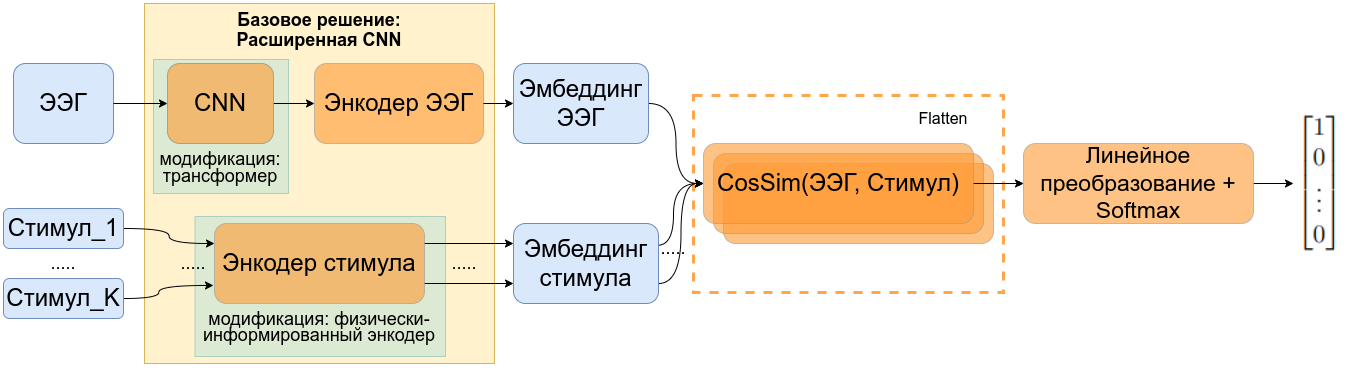
\includegraphics[scale=0.3]{model_architecture.png}
        \caption{Архитектура модели. Базовое решение представляет собой расширенную сверточную нейросеть в качестве энкодера ЭЭГ-сигнала и стимулов, а также обычную сверточную нейросеть для пространсвтенного преобразования ЭЭГ-сигнала. Получаются скрытые представления ЭЭГ-сигнала и стимулов, считается их близость и находится истинный стимул. Предлагается использовать трансформера-кодировщика, чтобы уменьшить число каналов ЭЭГ-сигнала до подачи в расширенную сверточную нейросеть и физико-информированные энкодеры для получения эмбеддингов стимулов. После получения эмбеддингов стимулов аналогично определятся истинный стимул, как наиболее близкий к эмбеддингу ЭЭГ-сигнала.}
        \label{model}
    \end{figure}

\section{Описание модели}
    Архитектура модели представлена на рис.~\ref{model}. Модель получает на вход ЭЭГ-сигнала $\mathbf{X}$ и набор стимулов $\mathbf{s}_1, \dots, \mathbf{s}_K$. В начале снижается размерность ЭЭГ-сигнала от 64 до 8 и подается на вход энкодеру ЭЭГ. Также и стимулы проходят через энкодер и, получив представление ЭЭГ-сигнала $\mathbf{E}$ и представления стимулов $\mathbf{Z}_1, \dots, \mathbf{Z}_K$ в латентном пространстве $\mathbb{R}^{16 \times \mathcal{T}}$, считается их близость по формуле $\mathbf{C}_k = \operatorname{CosSim}(\mathbf{E}, \mathbf{Z}_k) = \mathbf{E} \mathbf{Z}_k^T$ для $k \in \{1, \dots, K\}$. Далее для каждой матрицы производится линейное преобразование $c_k = \mathbf{w}^T \mathbf{r}_k + b$, где $\mathbf{r}_k$~--- матрица $\mathbf{C}_k$ в виде вектора, $\mathbf{w} \in \mathbb{R}^{256}$~--- вектор коэффициентов и $b$~--- свободный член. Итоговое распределение вероятностей получается, как $\mathbf{p} = \operatorname{SoftMax}\left( \left[c_1, \dots, c_K \right]^T \right)$.

    \subsection{Базовая модель}
    В базовом решении для пространственного преобразования ЭЭГ-сигнала используется сверточная нейронная сеть. Одномерная свертка с ядром $1 \times 1$ и 8 фильтрами объединяет информацию по всем 64 каналам и уменьшает размерность до 8. \par 
    Структура энкодеров ЭЭГ и стимулов одинаковая, но они имеют разные веса. Эти энкодеры состоят из $n$ блоков расширенной сверточной нейросети. Блоки идентичные и каждый из них имеет 16 фильтров с ядрами $3 \times 3$. В пределах одного блока, в каждом слое ядро имеет свой коэффициент расширения равное $3^{m-1}$.\par 
    % В данном блоке 8 фильтров с ядром $1 \times 1$ 
    % В базовом решении используется расширенная сверточная нейросеть, в качестве энкодера ЭЭГ и стимулов с общими весами. Отметим, что все свертки одномерные. В начале сверточный слой с 8 фильтрами  и ядром $1 \times 1$ объединяет информацию по всем 64 каналам и уменьшает размерность. Преобразованная матрица $\mathbf{X}_1 = \mathrm{Conv}(\mathbf{X}, K_1)$, где $K_1$~--- ядро слоя, а $\mathbf{X}$~--- ЭЭГ-сигнал, имеет размерность $8 \times T$. Энкодер ЭЭГ в базовом решении представляет собой $n$ блоков расширенной сверточной сети. Блоки идентичные и каждый из них имеет 16 фильтров с ядрами $3 \times 3$. Ядра на каждом слое в пределах одного блока будут разными. Например, для слоя $L_m$ ядро $K_2^m$ будет иметь коэффициент расширения равному $3^{m-1}$. Описанный энкодер ЭЭГ дает скрытое представление матрицы $\mathbf{X}_1$, обозначим его $\mathbf{E}$, в латентном пространстве $\mathbb{R}^{16 \times T'}$. Аналогично получаем скрытое представление стимулов $\mathbf{P}_1, \dots, \mathbf{P}_K$ в том же латентном пространстве, за исключением того, что стимулы сразу проходят через $n$  блоков энкодера.

    \subsection{Предлагаемые решения}
    Предлагается заменить блок со сверточной нейросетью на трансфоремр-кодировщик~\citep{vaswani2023attention}, который за счет механизма внимания сможет улавливать долгосрочные зависимости в ЭЭГ-сигнале. Трансформер-кодировщик состоит из двух слоев. Первый представляет собой многомерное внимание, а второй --- полносвязная 2х-слойная нейросеть (FFN). После каждого слоя используется сквозная связь и нормализуется выход. Скрытый слой в FFN имеет размерность 32. \par 
    Модели автоматического распознавания речи (Automatic Speech Recognition) могут извлечь разные детали речи, по типу фонем и частот. В связи с этим было решено использовать современные модели ASR, такие как Wav2Vec 2.0~\citep{baevski2020wav2vec} и Whisper~\citep{radford2022robust}, в качестве энкодера стимула.
    \begin{itemize}
        \item Wav2Vec 2.0. Архитектура модели состоит из сверточной нейронной сети и трансформера. Сверточная нейронная сеть извлекает высокоуровневые признаки из аудио, а трансформер захватывает контекстную информацию.
        \item Whisper. Модель на основе трансформера с кодировщиком и декодировщиком. Она отображает последовательность признаков спектрограммы речи на последовательность текстовых токенов. Сначала исходные аудиовходы преобразуются в mel-спектрограмму с помощью извлекателя признаков. Затем трансформер-кодировщик, формирует последовательность скрытых состояний. Наконец, декодер авторегрессивно предсказывает текстовые токены.
    \end{itemize}
    

\section{Вычислительный эксперимент}
    
\subsection{Данные}
    Эксперимент проверялся на данных~\citep{K3VSND_2023}. Они представляли собой выборку из 85 человек. Все участники прослушали 6, 7, 8 или 10 стимулов на датском языке, каждая из которых имеет примерную продолжительность 15 мин. После прослушивания участников спрашивали про содержания аудиофрагмента. Это было с целью мотивировать участников обращать внимания во время прослушивания.

    Стимулы были разделены на следующие категории:

    \begin{itemize}
        \item Справочные аудиокниги
        \item Аудиокниги для детей и взрослых. Если длина превышала 15 мин, то аудиокнига делилась на части
        \item Аудиокниги с шумом
        \item Подкасты про ответы на научные вопросы
        \item Подкасты с видео
    \end{itemize}

    Были использованы обработанные данные аудифрагментов и ЭЭГ-сигналов, а также необработанные аудиофрагменты, с частотами дискретизации равными  64 Гц и 48000 Гц соответственно. Отметим также, что обработанные аудиофрагменты представляют собой огибающую сигнала (рис.~\ref{envelope_spectr}).
    \begin{figure}[!h]
        \centering
        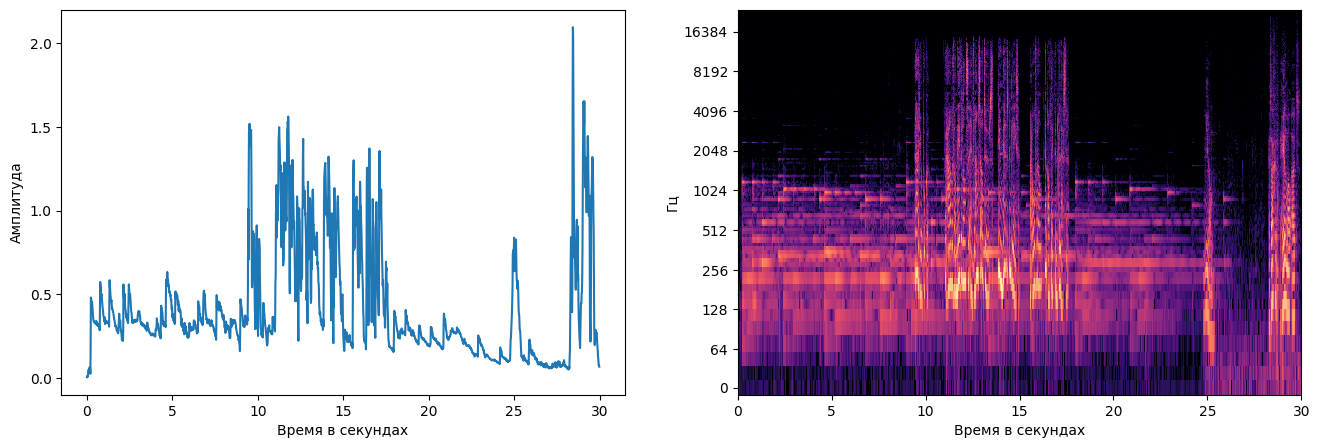
\includegraphics[width=1\textwidth]{env_spectr.png}
        \caption{Пример огибающей(слева) и спектрограммы(справа) одного и того же аудиофрагмента продолжительностью 30 секунд.}
        \label{envelope_spectr}
    \end{figure}

    \subsection{Описание эксперимента}    
    Для эксперимента была выделена случайная подвыборка из 25 участников с равным количеством мужчин и женщин, и аудиофрагменты, которые они слушали, а также соответсвтующие записи ЭЭГ-сигналов. Всего 183 пар (ЭЭГ-сигнал, стимул). \par  
    Так как исходные обработанные ЭЭГ-сигналы и аудиофрагменты слишком велики, они были разбиты на окна фиксированной длины. Для каждой пары окон (ЭЭГ-сигнал, истинный стимул) были сгенерированы $K-1$ ложных стимулов той же длины, что и длина окна. Далее для обеспечения сбалансированности классов были созданы $K-1$ копий каждого объекта, со смещением истинного стимула. \par 
    С учетом языка аудиосигналов было решено взять предобученную модель wav2vec2-base-960h-phoneme-reco-dutch и whisper-small. Для работы с ASR моделями необработанные аудиофрагменты переводились в подходящий вид. Для каждого аудио с помощью модели создавался эмбеддинг, который потом выравнивался, по уже готовым данным. \par
    В эксперименте ширина окна была взята равной 5 секунд с шагом 1 секунда. Количество стимулов $K=5$, то есть один истинный стимул и четыре ложных. Эксперимент проводился в $10$ эпох, а размер батча составлял 64 элементов. В качестве метрики взята среднее по участникам долей правильных ответов. 
    
    Обозначим множество классов, как $\{0, \dots, K-1\}$. Учитывая это, метрика качества вычисляется по формуле
$$
    Score = \frac{1}{22} \sum_{i=1}^{22} \frac{1}{l_i} \sum_{j=1}^{l_i} \left[ y^i_j = \text{pred}^i_j\right],
$$
где $y^i_j \in \{0, \dots, K-1\}$~--- метка объекта, $l_i$~--- количество пар ЭЭГ-стимул для $i$-го участника, а $\text{pred}^i_j$~--- предсказание модели на объекте $j$.

    \subsection{Результаты эксперимента}
    Результаты экспериментов приведены в таблице~\ref{results_table}. Видно, что комбинирование трансформера-кодировщика с физико-информированными моделями Wav2Vec 2.0 и Whisper-small дали наилучшие результаты. \par 
    {\renewcommand{\arraystretch}{1.3}%
    \begin{table}[h!]
        \centering
        \begin{tabular}{|c|c|} \hline 
            Model & Score (\%) \\ \hline
            Baseline & 47.68 $\pm$ 11.75 \\ 
            Transformer Encoder & 48.15 $\pm$ 10.33 \\ 
            Wav2Vec2 & 47.92 $\pm$ 11.54 \\   
            Whisper-small & 48.04 $\pm$ 9.85 \\   
            Transformer Encoder + Wav2Vec2 & \bm{48.70} \; $\pm$ 9.44 \\ 
            Transformer Encoder + Whisper-small & 48.36 $\pm$ 9.24\\ \hline
        \end{tabular}
        \vspace{5pt}
        \caption{Оценка качества на использованных моделях.}
        \label{results_table}
    \end{table}}
    \newpage

    По предсказаниям на тестовых данных построим график boxplot~\ref{results_boxplot} для каждой модели. По оси ординат указано доля правильных ответов для каждого участника. \par 
    \begin{figure}[h!]
        \centering
        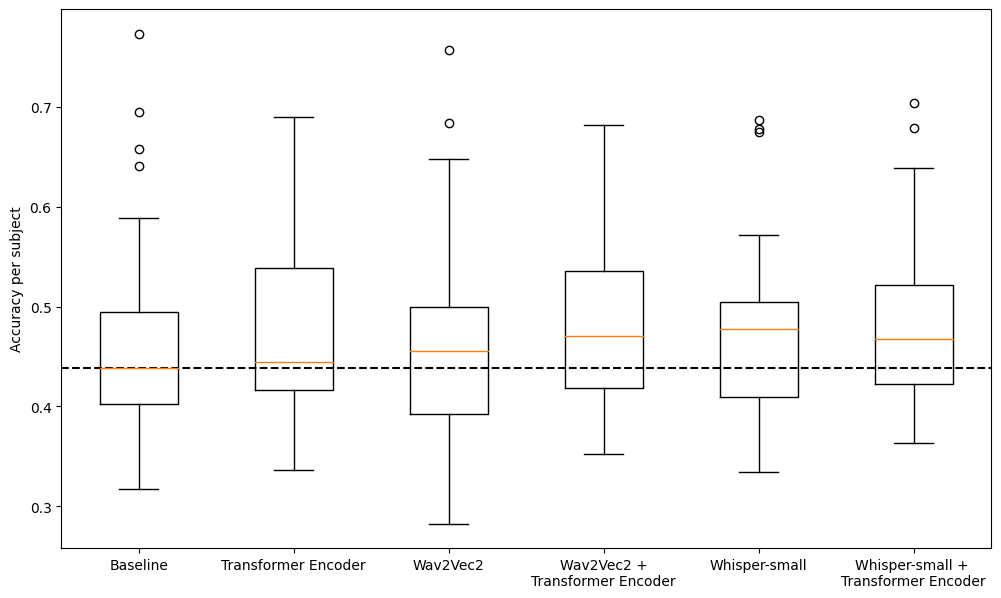
\includegraphics[width=0.9\textwidth]{boxplot_results.png}
        \caption{График boxplot построенный на тестовых данных}
        \label{results_boxplot}
    \end{figure}
    Как можно видеть по графику, межквартильный размах расположен выше базового решения у комбинированных моделей и трансформера-кодировщика. Согласно графику, наибольший прирост качества получается за счет трансформера-кодировщика и модели Wav2Vec 2.0. Это объясняется тем, что для построения эмбеддингов была взята предобученная модель Wav2Vec 2.0, которая была настроена на датский язык. Использование эмбеддингов модели Whisper-small чуть уступает по качеству, так как предобученная модель является общей для всех языков и не настраивалась именно на дасткий язык.

\section{Заключение}
Эксперименты показали, что использование трансформеров и физико-информированных моделей в качестве энкодеров приводит к улучшению качества классификации истинного стимула для ЭЭГ-сигнала. Этот результат подтверждает гипотезу о том, что интеграция физических законов может улучшить точность их классификации. Эти результаты имеют важное значение для практических приложений, таких как разработка интерфейсов мозг-компьютер. 
%Повышенная точность классификации, достигаемая за счет использования физико-информированных моделей и трансформера, может положительно повлиять на точность таких систем, что является важным шагом в развитии методов анализа и интерпретации ЭЭГ-сигналов.

В дальнейшем планируется провести эксперименты с разными размерностями скрытого состояния физико-информированных энкодеров. Ожидается найти баланс между информацией инкапсулируемой в эмебеддинге и её размерностью, так как большие размерности требуют огромных затрат памяти.

\bibliographystyle{plain}
\bibliography{Nabiev2024SignalToAudio}

\end{document}